%%% Template originaly created by Karol Kozioł (mail@karol-koziol.net) and modified for ShareLaTeX use

\documentclass[a4paper,11pt]{article}

\usepackage[T1]{fontenc}
\usepackage[utf8]{inputenc}
\usepackage{float}
\usepackage{xcolor}
\usepackage{parskip}
\usepackage{tgtermes}
\usepackage{graphicx,wrapfig}
\usepackage[
pdftitle={Math Assignment}, 
pdfauthor={Lucas Varela, Universidad de los Andes},
colorlinks=true,linkcolor=blue,urlcolor=blue,citecolor=blue,bookmarks=true,
bookmarksopenlevel=2]{hyperref}
\usepackage{amsmath,amssymb,amsthm,textcomp}
\usepackage{enumerate}
\usepackage{multicol}
\usepackage{tikz}
\definecolor{pr}{HTML}{FF6961}
\definecolor{pb}{HTML}{779ecb}
\usepackage{hyperref}

\definecolor{pg}{HTML}{77DD77}

\usepackage{geometry}
\geometry{total={210mm,297mm},
left=25mm,right=25mm,%
bindingoffset=0mm, top=20mm,bottom=20mm}


\linespread{0.9}

\newcommand{\linia}{\rule{\linewidth}{0.5pt}}

% custom theorems if needed


% my own titles
\makeatletter
\renewcommand{\maketitle}{
\begin{center}
\vspace{2ex}
{\huge \textsc{\@title}}
\vspace{1ex}
\\
\linia\\
\@author \hfill \@date
\vspace{4ex}
\end{center}
}
\makeatother
%%%

% custom footers and headers
\usepackage{fancyhdr,lastpage}
\pagestyle{fancy}
\lhead{}
\chead{}
\rhead{}
\lfoot{Solución problema Kleppner 4.23}
\cfoot{}
\rfoot{Page \thepage\ /\ \pageref*{LastPage}}
\renewcommand{\headrulewidth}{0pt}
\renewcommand{\footrulewidth}{0pt}
%

%%%----------%%%----------%%%----------%%%----------%%%

\begin{document}

\title{Solución problema Kleppner 4.23}

\author{Física I}

\date{}

\maketitle

\color{blue}
\setlength\intextsep{-10pt}


\begin{wrapfigure}{r}{3.0cm}
	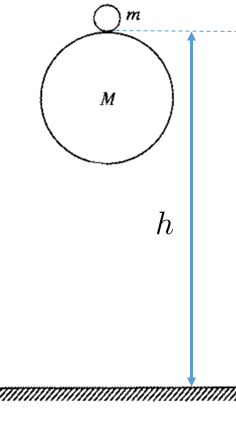
\includegraphics[scale=0.7]{./im/1}
\end{wrapfigure}





\color{pb}
\textbf{Kleppner 4.23} \color{black} Una bola de masa $M$ y otra de masa $m$ se sueltan juntas desde una altura $h$ del suelo ($h$ se mide desde el suelo hasta el punto de contacto entre las bolas). Encuentre la altura máxima que alcanza la bola pequeña sabiendo que $m$ es mucho menos masiva que $M$ ($m\ll M$). Suponga que todas las colisiones son elásticas.




\begin{center}
	\color{pb}
\textbf{Solución}
\color{black}
\end{center}
Primero se calcula la rapidez de la pelota al llegar al suelo. Para una caída libre conocemos la rapidez en función de la altura desde que se suelta $h$:

$$v^2 = 2gh$$


Esta también es la rapidez con la que llega la pelota pequeña (recuerde que en caída libre la velocidad final no depende de la masa). Ahora como la colisión con el piso es elástica, la energía antes y después de la colisión es la misma, por lo que la pelota $M$ rebota y sale con la misma rapidez pero con la dirección opuesta. Entonces vemos que después de que la pelota $M$ rebota se tiene la siguiente situación mostrada en el dibujo.

\vspace{1cm}

\begin{figure}[H]
	\centering
	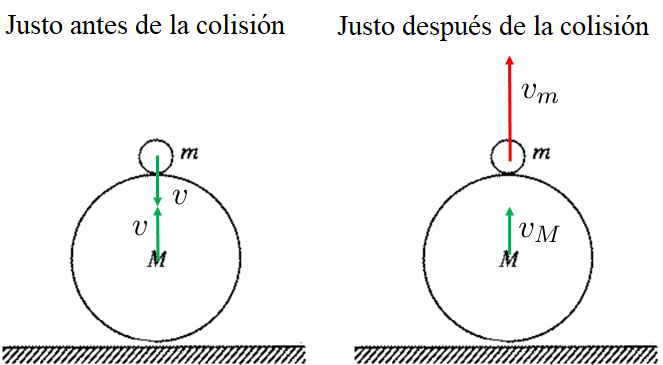
\includegraphics[scale=1]{./im/2}
	\caption{Justo antes y después de la colisión entre las bolas. En el momento justo antes la bola grande ya rebotó con en el piso.}
\end{figure}

\vspace{0.5cm}

Entonces ambas pelotas se mueven con la misma rapidez y dirección opuesta. Por lo tanto justo antes de la colisión entre las bolas se tiene el siguiente momento lineal en la dirección $y$:

$$ p_{i} = M v - m v = (M-m)v$$

Y justo después:

\begin{equation}
p_f = M v_M + m v_m
\end{equation}



Dado que es una colisión elástica rectilínea, tenemos la siguiente relación para la velocidad relativa antes y después de la colisión:

\begin{equation}
v_{M_i} -v_{m_i} = -(v_{M_f} -v_{m_f})
\end{equation}

Se reemplaza en la ecuación anterior las velocidades que se conocen:

\begin{equation}
v - (-v) = -(v_M - v_m)
\end{equation}

y se despeja $v_M$:

\begin{equation}
v_M = v_m - 2v \label{vM}
\end{equation}

Para despejar $v_m$ necesitamos otra ecuación que sale de plantear la conservación del momento lineal:

\begin{equation}
(M-m)v = M v_M + m v_m
\end{equation}

Reemplazamos la expresión para $v_M$ (ecuación \ref{vM}) en la relación anterior para despejar $v_m$:



\begin{align*}
(M-m)v = M (v_m - 2v) + m v_m\\
(M-m)v = Mv_m - 2Mv + m v_m\\
(3M-m)v = (M+m) v_m
\end{align*}



Finalmente se obtiene:

\begin{equation}
v_m = \frac{3M-m}{M+m} v
\end{equation}

Si miramos $M \gg m$, podemos simplificar la expresión anterior aún más. Podemos decir que ya que $M$ es mucho más grande que $m$, se tiene que $m/M \approx 0$. Veamos que implica eso en nuestra expresión para $v_m$:

\begin{equation}
v_m = \frac{3M-m}{M+m} v =  \frac{M}{M}\frac{3-m/M}{1+m/M} v \approx 3 v
\end{equation}

La pelota pequeña sale disparada con una rapidez $3v$ que nos da una altura final $h_f$:

\begin{equation}
h_f = \frac{v_m^2}{2g} = 9\frac{v^2}{2g} =  9 h
\end{equation}

El resultado anterior puede parecer equivocado pero podemos confirmar su veracidad con un experimento:


\url{https://youtu.be/2UHS883_P60?t=106}


\vspace{1cm}

\begin{figure}[H]
	\centering
	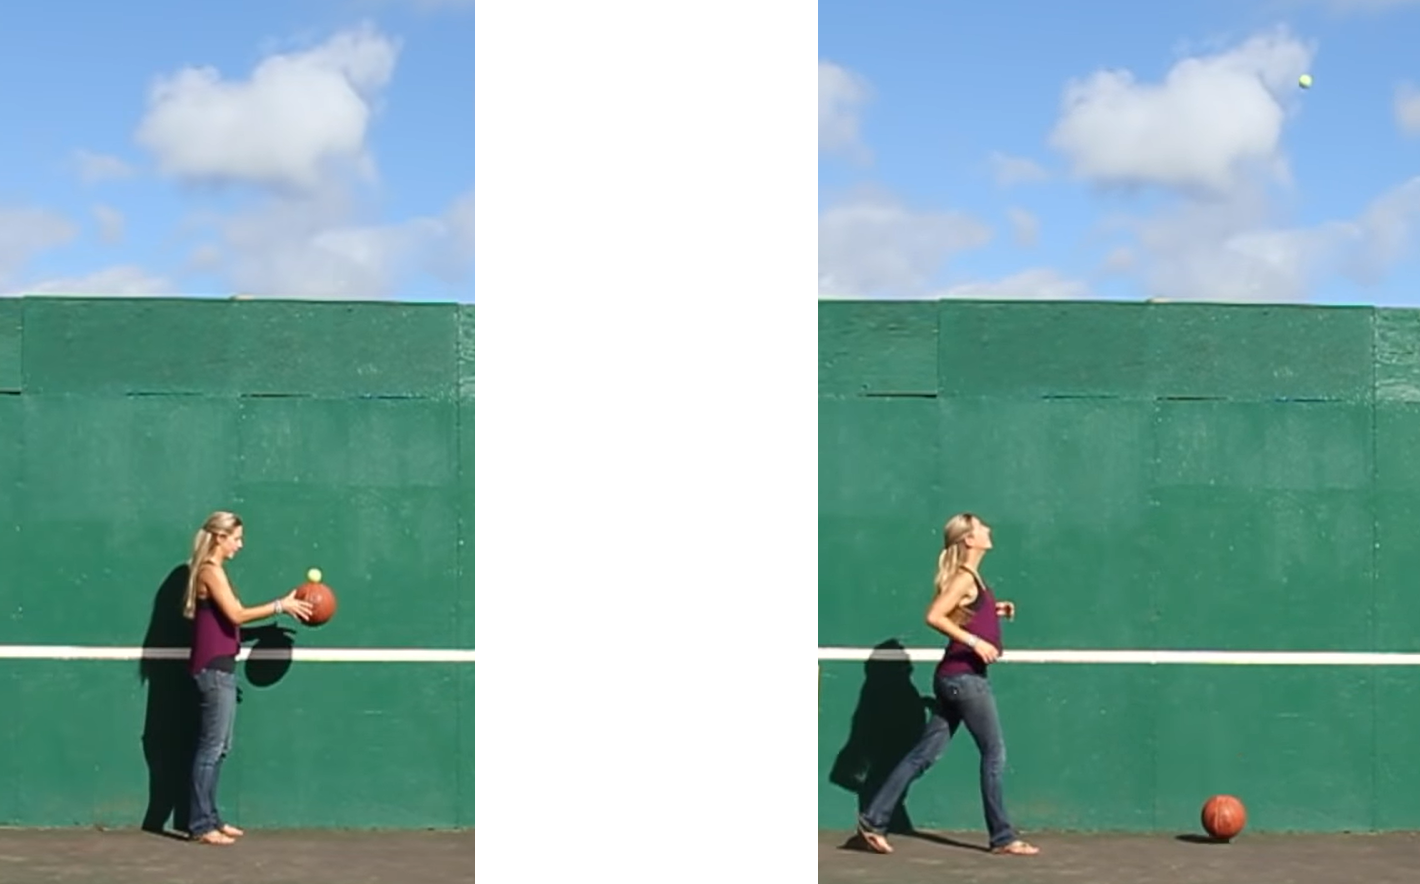
\includegraphics[width=\linewidth]{./im/girl1}
	\caption{Justo antes y después de la colisión entre las bolas. La pelota pequeña alcanza una gran altura. En este experimento claramente no se alcanza nueve veces la altura original y esto se debe a la fricción con el aire y que la colisión no fue perfectamente rectilíneo (note que la pelota de tenis no está alienada con la pelota de baloncesto. Finalmente, en este caso se tiene $m/M \approx 0.09$ y si tomamos eso en cuenta la altura final disminuye a aproximadamente $7h$. Imágenes tomadas del vídeo de Physics Girl: \url{https://youtu.be/2UHS883_P60?t=106}}
\end{figure}



\end{document}
